% Cumulative Monday/Wednesday lecture notes. Compile with pdfLaTeX (two passes).
% All figures are native PGFPlots; no images, data files, or shell escape.
% Source lineage: archived instructor Chapter 5 notes through end of chapter.
% Updated September 28, 2026 for Wednesday read-ahead. Seeded simulation data inline.
\documentclass[11pt,letterpaper]{article}
\usepackage[T1]{fontenc}
\usepackage[utf8]{inputenc}
\usepackage{lmodern}
\usepackage[margin=0.9in,headheight=15pt]{geometry}
\usepackage{amsmath,amssymb}
\usepackage{microtype}
\usepackage{xcolor}
\usepackage{booktabs,tabularx,array}
\usepackage{enumitem}
\usepackage[most]{tcolorbox}
\usepackage{pgfplots}
\usepackage{titlesec}
\usepackage{fancyhdr}
\usepackage{hyperref}
\pgfplotsset{compat=1.18}

\definecolor{ink}{HTML}{193447}
\definecolor{teal}{HTML}{246E78}
\definecolor{pale}{HTML}{F1F6F7}
\definecolor{rose}{HTML}{A84450}
\definecolor{gold}{HTML}{986019}
\hypersetup{colorlinks=true,linkcolor=teal,urlcolor=teal,
  pdftitle={Chapter 5: Independence and Discrete Counting Models},
  pdfauthor={Zan Ahmad}}
\titleformat{\section}{\Large\bfseries\color{ink}}{\thesection}{0.65em}{}
\titleformat{\subsection}{\large\bfseries\color{teal}}{\thesubsection}{0.65em}{}
\titlespacing*{\section}{0pt}{2.0ex plus 1ex}{1.0ex}
\titlespacing*{\subsection}{0pt}{1.7ex plus 0.6ex}{0.6ex}
\setlength{\parindent}{0pt}
\setlength{\parskip}{0.55em}
\setlength{\emergencystretch}{2em}
\setlist{topsep=0.35em,itemsep=0.2em,parsep=0pt}
\renewcommand{\arraystretch}{1.25}
\newcolumntype{L}{>{\raggedright\arraybackslash}X}
\newcommand{\E}{\mathbb{E}}
\newcommand{\Prob}{\mathbb{P}}
\DeclareMathOperator{\Var}{Var}
\DeclareMathOperator{\Cov}{Cov}
\DeclareMathOperator{\Bernoulli}{Bernoulli}
\DeclareMathOperator{\Bin}{Bin}
\newcommand{\Ssym}{\mathrm{S}}
\newcommand{\Fsym}{\mathrm{F}}
\newtcolorbox{keyidea}[1]{enhanced,breakable,colback=pale,colframe=teal,
  boxrule=0.5pt,arc=1.5mm,left=9pt,right=9pt,top=6pt,bottom=6pt,
  title={#1},fonttitle=\bfseries,coltitle=white,colbacktitle=teal}
\newtcolorbox{careful}[1]{enhanced,breakable,colback=rose!4,colframe=rose!65,
  boxrule=0.5pt,arc=1.5mm,left=9pt,right=9pt,top=6pt,bottom=6pt,
  title={#1},fonttitle=\bfseries,coltitle=white,colbacktitle=rose}
\pagestyle{fancy}
\fancyhf{}
\fancyhead[L]{\small EN.553.211 \enspace Chapter 5 notes}
\fancyhead[R]{\small September 28 and 30, 2026}
\fancyfoot[C]{\small\thepage}
\renewcommand{\headrulewidth}{0.3pt}

\begin{document}
\begin{center}
{\small\sffamily\color{teal} PROBABILITY \& STATISTICS FOR LIFE SCIENCES}\par
\vspace{0.5em}
{\LARGE\bfseries\color{ink} Independence and Discrete Counting Models}\par
\vspace{0.3em}
{\large Bernoulli, binomial, hypergeometric, and Poisson}\par
\vspace{0.65em}
{\large Zan Ahmad}\par
September 28 and 30, 2026 \quad\textbullet\quad EN.553.211
\end{center}

\begin{keyidea}{Purpose and standing assumptions}
These notes continue from the properties of expectation and variance,
develop independence through centered deviations, and build counting models
from individual trials. Monday's material leads to the cereal-box example.
The Wednesday continuation begins at \hyperref[wed-start]{cereal part (b),
page~\pageref{wed-start}}, derives binomial moments, contrasts sampling with
and without replacement, and continues through hypergeometric and Poisson
models to the end of Chapter 5.

All random variables in this article are \textbf{discrete and have finite
second moments}. In particular, every expectation, variance, and covariance
used below exists. Write $\mu_X=\E[X]$ and $\mu_Y=\E[Y]$.
The notation $\Var(X)$ means the same thing as $V(X)$ in the course slides.
\end{keyidea}

The main thread is a question: \emph{When may we add expectations, when may
we add variances, and how do those facts help us understand a count of
successes?} Keep the distinction between an individual outcome, a random
count, and the probability of that count visible throughout.

{\small\setcounter{tocdepth}{1}\tableofcontents}
\clearpage

\section{Independence: learning one value leaves the other distribution unchanged}
\label{independence-start}

Two random variables $X$ and $Y$ are independent when every pair of values
has a joint probability that factors into its two marginal probabilities:
\begin{keyidea}{Definition of independence}
\[
\boxed{\Prob(X=x,Y=y)=\Prob(X=x)\Prob(Y=y)
\quad\text{for every pair }(x,y).}
\]
The word \emph{every} matters. One factorization for one pair does not
establish independence of the random variables.
\end{keyidea}

Here $\Prob(X=x,Y=y)$ means the probability that \emph{both} equalities
hold. A marginal probability, such as $\Prob(Y=y)$, describes one variable
without conditioning on the other. If $\Prob(X=x)>0$, independence gives
\begin{align*}
\Prob(Y=y\mid X=x)
 &=\frac{\Prob(X=x,Y=y)}{\Prob(X=x)}
 &&\text{definition of conditional probability}\\
 &=\frac{\Prob(X=x)\Prob(Y=y)}{\Prob(X=x)}
 &&\text{independence}\\
 &=\Prob(Y=y).
\end{align*}
Thus, after learning $X=x$, the probabilities assigned to the possible
values of $Y$ stay the same. The corresponding statement also holds with
$X$ and $Y$ reversed whenever the conditioning probability is positive.

Conversely, if the conditional distribution of $Y$ is unchanged for every
$x$ with positive probability, multiplying by $\Prob(X=x)$ recovers the
joint-probability definition. Values of $x$ with probability zero cause no
problem: all their joint probabilities are zero as well.

\begin{careful}{An information statement, not a causal statement}
Independence describes a probability distribution. It says that learning
one value does not change the distribution of the other. It does not, by
itself, establish whether one physical process causes or influences another.
\end{careful}

\section{Linearity, products, and covariance}

\subsection{Expectation is linear without independence}

For constants $a,b,c$, we always have
\[
\boxed{\E[aX+bY+c]=a\E[X]+b\E[Y]+c.}
\]
The two random variables may be independent, strongly related, or even the
same random variable. None of those possibilities changes this rule.
For example, $\E[X+X]=2\E[X]$ is still linearity.

One way to see why dependence does not obstruct addition is to use the
joint probability mass function. Summing over all possible values,
\begin{align*}
\E[X+Y]
 &=\sum_x\sum_y(x+y)\Prob(X=x,Y=y)\\
 &=\sum_x x\underbrace{\sum_y\Prob(X=x,Y=y)}_{\Prob(X=x)}
   +\sum_y y\underbrace{\sum_x\Prob(X=x,Y=y)}_{\Prob(Y=y)}\\
 &=\E[X]+\E[Y].
\end{align*}
We only added the joint probabilities over the other variable's possible
values. We did not factor the joint probability into a product.

\subsection{Independence lets an expected product factor}

For a product, a different step is needed. If $X$ and $Y$ are independent,
\begin{align*}
\E[XY]
 &=\sum_x\sum_y xy\Prob(X=x,Y=y)\\
 &=\sum_x\sum_y xy\Prob(X=x)\Prob(Y=y)
 &&\text{independence is used here}\\
 &=\sum_x x\Prob(X=x)\left(\sum_y y\Prob(Y=y)\right)\\
 &=\left(\sum_x x\Prob(X=x)\right)
   \left(\sum_y y\Prob(Y=y)\right)\\
 &=\E[X]\E[Y].
\end{align*}
The inner sum no longer depends on $x$, so it can be taken outside the
outer sum. Finite second moments ensure that these sums can be rearranged:
in particular, $2|XY|\le X^2+Y^2$ gives $\E[|XY|]<\infty$.

\begin{keyidea}{Two rules with different requirements}
\[
\begin{aligned}
\E[X+Y]&=\E[X]+\E[Y] &&\text{always},\\
\E[XY]&=\E[X]\E[Y] &&\text{if $X$ and $Y$ are independent}.
\end{aligned}
\]
Independence is sufficient for the product rule. We will soon see that it
is not necessary.
\end{keyidea}

\subsection{Covariance records the expected product of deviations}

The centered values $X-\mu_X$ and $Y-\mu_Y$ tell us how far each variable
lies above or below its own mean. Their product is positive when their
signs agree, negative when the signs differ, and zero when either deviation
is zero. Covariance averages these products:
\[
\Cov(X,Y)=\E[(X-\mu_X)(Y-\mu_Y)].
\]
Expanding the expression gives a useful computational formula:
\begin{align*}
\Cov(X,Y)
 &=\E[XY-\mu_Y X-\mu_X Y+\mu_X\mu_Y]\\
 &=\E[XY]-\mu_Y\E[X]-\mu_X\E[Y]+\mu_X\mu_Y\\
 &=\E[XY]-\mu_X\mu_Y-\mu_X\mu_Y+\mu_X\mu_Y\\
 &=\boxed{\E[XY]-\E[X]\E[Y]}.
\end{align*}
The means are fixed numbers, so linearity permits pulling them outside
expectations. Independence was not used in this derivation.

\section{Why variances add: inspect the cross term}

\subsection{Center first, then expand}

Set
\[
A=X-\E[X],\qquad B=Y-\E[Y].
\]
These centered deviations have mean zero:
\[
\E[A]=\E[X]-\E[X]=0,\qquad \E[B]=0.
\]
The expectations of their squares recover the variances,
$\E[A^2]=\Var(X)$ and $\E[B^2]=\Var(Y)$, while their expected product is
$\E[AB]=\Cov(X,Y)$.

Linearity gives $\E[X+Y]=\E[X]+\E[Y]$, so the deviation of the sum from
its mean is exactly $A+B$. Now expand the square before taking averages:
\begin{align*}
\Var(X+Y)
 &=\E\!\left[\bigl((X+Y)-\E[X+Y]\bigr)^2\right]\\
 &=\E[(A+B)^2]\\
 &=\E[A^2+2AB+B^2]\\
 &=\E[A^2]+2\E[AB]+\E[B^2]\\
 &=\boxed{\Var(X)+\Var(Y)+2\Cov(X,Y)}.
\end{align*}
The extra term is not a technical afterthought: it measures whether the
two deviations tend to reinforce or oppose one another.

For a difference, the centered deviation is $A-B$ instead:
\begin{align*}
\Var(X-Y)
 &=\E[(A-B)^2]\\
 &=\E[A^2-2AB+B^2]\\
 &=\boxed{\Var(X)+\Var(Y)-2\Cov(X,Y)}.
\end{align*}
The individual squared terms remain positive; it is the \emph{cross term}
whose sign changes. We do not subtract $\Var(Y)$.

\subsection{The precise job of independence}

If $X$ and $Y$ are independent, their centered versions $A$ and $B$ are
also independent: subtracting a fixed number simply relabels the possible
values. The product rule therefore gives
\[
\E[AB]=\E[A]\E[B]=0\cdot0=0.
\]
This is why the cross term disappears. It does not require either
distribution to be symmetric.

\begin{keyidea}{Independent sums and differences}
When $X$ and $Y$ are independent,
\[
\boxed{\Var(X+Y)=\Var(X)+\Var(Y)},\qquad
\boxed{\Var(X-Y)=\Var(X)+\Var(Y)}.
\]
The same formulas also hold whenever their covariance is zero, even if
they are dependent.
\end{keyidea}

\subsection{Exactly what is equivalent to what?}

For two variables with finite second moments, the identities we have
derived show the exact equivalences
\begin{keyidea}{Equivalent statements for this pair of variables}
\[
\begin{gathered}
\Cov(X,Y)=0\\
\Updownarrow\\
\E[XY]=\E[X]\E[Y]\\
\Updownarrow\\
\Var(X+Y)=\Var(X)+\Var(Y)\\
\Updownarrow\\
\Var(X-Y)=\Var(X)+\Var(Y).
\end{gathered}
\]
Independence implies all four statements. None of them, by itself,
implies independence.
\end{keyidea}

There is an important distinction between a \emph{centered} product and a
product of arbitrary random variables. For the centered $A,B$ above,
$\E[AB]=\Cov(X,Y)$. To keep this separate from centering, use fresh names
$U,V$ for arbitrary random variables. In general,
\[
\E[UV]=\Cov(U,V)+\E[U]\E[V].
\]
Thus $\E[UV]=0$ holds exactly when the covariance and the product of the
means cancel:
\[
\Cov(U,V)=-\E[U]\E[V].
\]
Under independence, the covariance is zero, so $\E[UV]=0$ holds exactly
when at least one of $\E[U]$ and $\E[V]$ is zero. Without independence,
even having \emph{both} means zero is not enough.

\section{Examples and the many-variable rule}

\subsection{Zero covariance can hide dependence}

Let $X$ be uniform on $\{-1,0,1\}$ and define $Y=X^2$. There are three
possible joint outcomes, each with probability $1/3$:
\begin{center}
\begin{tabular}{rrrr}
\toprule
$X$ & $Y=X^2$ & $XY$ & Probability\\
\midrule
$-1$ & $1$ & $-1$ & $1/3$\\
$0$  & $0$ & $0$  & $1/3$\\
$1$  & $1$ & $1$  & $1/3$\\
\bottomrule
\end{tabular}
\end{center}
Read each expectation as a weighted average of its column:
\begin{align*}
\E[X]&=(-1)\frac13+0\frac13+1\frac13=0,\\
\E[Y]&=1\frac13+0\frac13+1\frac13=\frac23,\\
\E[XY]&=(-1)\frac13+0\frac13+1\frac13=0.
\end{align*}
Therefore
\[
\Cov(X,Y)=0-0\left(\frac23\right)=0.
\]
But knowing $X$ determines $Y$ completely. For example,
\[
\Prob(Y=0\mid X=0)=1
\quad\text{whereas}\quad
\Prob(Y=0)=\frac13.
\]
The conditional distribution changes, so the variables are dependent.
This one example also disproves the claim that
$\E[XY]=\E[X]\E[Y]$ implies independence. That equality checks one
weighted average; independence checks the entire joint distribution.

\subsection{Symmetry and zero means do not remove dependence}

Let $A$ take $-1$ and $1$ with equal probabilities and let $B=A$.
Both distributions are symmetric about zero, and
$\E[A]=\E[B]=0$. Nevertheless,
\[
AB=A^2=1\quad\text{on every outcome},\qquad \E[AB]=1.
\]
The deviations always have the same sign. Symmetry in each distribution
does not make the two variables independent and does not force their
expected product to vanish.

\subsection{Several variables: each pair contributes a cross term}

For $X_1,\ldots,X_n$, expand the square of the sum of their centered
deviations. Each squared term appears once; each distinct pair appears
twice. Consequently,
\[
\boxed{\Var\!\left(\sum_{i=1}^n X_i\right)
=\sum_{i=1}^n\Var(X_i)+2\sum_{1\le i<j\le n}\Cov(X_i,X_j).}
\]
The notation $i<j$ means that every pair is counted once. If the variables
are independent, all pairwise covariances are zero and the variances add.
In fact, \emph{pairwise independence} is sufficient for this variance
calculation, and pairwise zero covariance is sufficient as well.
For three or more variables, variance additivity for the total only says
that the \emph{sum} of the cross covariances is zero; individual nonzero
covariances can cancel.

\subsection{Two independent copies versus twice the same variable}

Suppose $X_1$ and $X_2$ are independent copies, each with variance
$\sigma^2$. Then
\[
\Var(X_1+X_2)=\sigma^2+\sigma^2=2\sigma^2.
\]
If we double one variable instead, we double every deviation from its mean:
\[
\Var(2X)=\E[(2X-2\E[X])^2]
=4\E[(X-\E[X])^2]=4\sigma^2.
\]
Equivalently, $\Cov(X,X)=\Var(X)=\sigma^2$, so adding $X$ to itself
includes the extra $2\sigma^2$ cross term.

\begin{center}
\begin{tabularx}{\linewidth}{@{}p{0.40\linewidth}L@{}}
\toprule
Relationship & What we may conclude\\
\midrule
Any $X,Y$ & Expectations add; variances include $2\Cov(X,Y)$.\\
Independent $X,Y$ & Expected products factor; covariance is zero; variances add.\\
$\Cov(X,Y)=0$ & Expected products factor and variances add; independence is not established.\\
Symmetric distributions with zero means & No general conclusion that $\E[XY]=0$.\\
Independent equal-variance copies & Variance of their sum is $2\sigma^2$.\\
Twice the same variable & Variance is $4\sigma^2$.\\
\bottomrule
\end{tabularx}
\end{center}

\section{One trial: the Bernoulli distribution}
\label{bernoulli-start}

\subsection{Code the outcome as zero or one}

A Bernoulli random variable records whether one specified event occurs.
We call the event a ``success'' and code it as $1$; otherwise the outcome
is called a ``failure'' and coded as $0$. These are neutral labels, not
judgments about whether an outcome is desirable.

Write $p\in[0,1]$ for the success probability and $q=1-p$ for the failure
probability. Then $X\sim\Bernoulli(p)$ has probability mass function
\begin{center}
\begin{tabular}{ccc}
\toprule
Outcome & Value $x$ & $\Prob(X=x)$\\
\midrule
Failure & $0$ & $q=1-p$\\
Success & $1$ & $p$\\
\bottomrule
\end{tabular}
\end{center}
The expectation is the probability-weighted average of these numerical
values:
\[
\boxed{\E[X]=0\cdot q+1\cdot p=p.}
\]
The mean equals $p$ because of the zero--one coding.

\subsection{Variance from squared deviations}

Since the mean is $p$, the two deviations are $0-p$ and $1-p=q$.
We square each deviation and weight it by the probability of its outcome:
\begin{center}
\begin{tabular}{ccccc}
\toprule
Value & Deviation & Squared deviation & Weight & Contribution\\
\midrule
$0$ & $-p$ & $p^2$ & $q$ & $p^2q$\\
$1$ & $1-p=q$ & $q^2$ & $p$ & $q^2p$\\
\bottomrule
\end{tabular}
\end{center}
Thus
\begin{align*}
\Var(X)
 &=(0-p)^2q+(1-p)^2p\\
 &=p^2q+q^2p\\
 &=pq(p+q) &&\text{factor out the common factor $pq$}\\
 &=\boxed{pq=p(1-p)} &&\text{because $p+q=1$}.
\end{align*}
The squares and the probability weights have different jobs: $p^2$ is
the squared deviation for outcome $0$, while $q$ is its probability.

\subsection{A second derivation using the zero--one coding}

For either possible outcome, $X^2=X$: both $0^2=0$ and $1^2=1$.
Consequently $\E[X^2]=\E[X]=p$. The variance shortcut gives
\[
\Var(X)=\E[X^2]-(\E[X])^2=p-p^2=p(1-p).
\]
Notice that $\E[X^2]=p$, whereas $(\E[X])^2=p^2$.
Taking a square before averaging and squaring an average are different
operations.

\subsection{When is a Bernoulli outcome most variable?}

At $p=0$, the outcome is certainly $0$; at $p=1$, it is certainly $1$.
In either case, the variance is zero because there is no uncertainty in
the outcome. To find the largest variance, regard
\[
V(p)=p(1-p)=p-p^2,\qquad 0\le p\le1,
\]
as a function of $p$. Its derivatives are
\[
V'(p)=1-2p,\qquad V''(p)=-2.
\]
The derivative is zero at $p=1/2$, and the negative second derivative
shows that this is a maximum. Comparing with the zero-variance endpoints,
\[
\boxed{\max_{0\le p\le1}p(1-p)=\frac14,
\quad\text{attained at }p=\frac12.}
\]
A trial is most uncertain when its two outcomes are equally likely.
The variance is $1/4$; the corresponding standard deviation is $1/2$.

\section{Repeated trials: a binomial count}
\label{binomial-start}

Fix a number of trials $n$. Each trial has two outcomes, the same success
probability $p$, and the trials are \emph{mutually independent}. Introduce
an indicator for each trial:
\[
X_i=\begin{cases}
1,&\text{trial $i$ is a success},\\
0,&\text{trial $i$ is a failure}.
\end{cases}
\qquad X_i\sim\Bernoulli(p).
\]
The total number of successes is
\[
\boxed{S=X_1+\cdots+X_n\sim\Bin(n,p).}
\]
The symbol $S$ here is a random \emph{count}, taking values
$0,1,\ldots,n$. It is not a probability. We use the upright letters
$\Ssym$ and $\Fsym$ for the success and failure symbols in a sequence.

The model assumptions each matter: a fixed number of trials, independent
outcomes, and a common success probability. Pairwise independence was
enough to remove covariance terms, but the binomial model uses mutual
independence to multiply probabilities along an entire outcome sequence.

\subsection{Three coin flips: exactly two heads}

Suppose three independent flips each have head probability $p$. There
are three distinct sequences with exactly two heads:
\begin{center}
\begin{tabular}{cc}
\toprule
Sequence & Probability\\
\midrule
$\mathrm{HHT}$ & $p\cdot p\cdot q=p^2q$\\
$\mathrm{HTH}$ & $p\cdot q\cdot p=p^2q$\\
$\mathrm{THH}$ & $q\cdot p\cdot p=p^2q$\\
\bottomrule
\end{tabular}
\end{center}
Independence lets us multiply within each sequence. The three sequences
are disjoint outcomes, so we add their probabilities:
\[
\Prob(\text{exactly two heads})=p^2q+p^2q+p^2q=3p^2q.
\]
For a fair coin, this is $3(1/2)^2(1/2)=3/8$.
The factor $3$ counts which positions contain the two heads.

\section{Count the positions, then attach their probabilities}
\label{counting-start}

\subsection{Five slots and exactly two successes: all ten arrangements}

First ignore probabilities and ask only where the successes can go.
Group the possible strings by the location of their first success:
\begin{center}
\begin{tabular}{clc}
\toprule
First success in slot & Strings & Number\\
\midrule
$1$ & \texttt{SSFFF}, \texttt{SFSFF}, \texttt{SFFSF}, \texttt{SFFFS} & $4$\\
$2$ & \texttt{FSSFF}, \texttt{FSFSF}, \texttt{FSFFS} & $3$\\
$3$ & \texttt{FFSSF}, \texttt{FFSFS} & $2$\\
$4$ & \texttt{FFFSS} & $1$\\
\midrule
 & Total & $4+3+2+1=10$\\
\bottomrule
\end{tabular}
\end{center}
Once the two success positions are chosen, every other slot must contain
a failure. There is no further choice to make for those remaining slots.

\subsection{Why dividing by a factorial removes overcounting}

Temporarily distinguish the two successes by calling them
$\Ssym_A$ and $\Ssym_B$. There are five choices for the position of
$\Ssym_A$ and four remaining choices for the position of $\Ssym_B$:
\[
5\cdot4=20\quad\text{placements of the labeled successes}.
\]
But the actual experiment records only success or failure, not an
$A$ or $B$ label. For example,
\[
\Ssym_A\,\Fsym\,\Ssym_B\,\Fsym\,\Fsym
\quad\text{and}\quad
\Ssym_B\,\Fsym\,\Ssym_A\,\Fsym\,\Fsym
\]
both become the same string \texttt{SFSFF} when the labels are erased.
Every success-position pattern was counted exactly $2!=2$ times.
Therefore the number of distinct success/failure strings is
\[
\binom{5}{2}=\frac{5\cdot4}{2!}=10.
\]
The division does not discard possible outcomes. It corrects how often
our temporary labeling counted each actual outcome.

For $k$ labeled successes in $n$ slots, the corresponding ordered count is
\[
n(n-1)\cdots(n-k+1).
\]
There are $k!$ ways to permute the labels among any fixed set of $k$
success positions. Dividing by this common overcount gives
\begin{align*}
\binom{n}{k}
 &=\frac{n(n-1)\cdots(n-k+1)}{k!}\\
 &=\boxed{\frac{n!}{k!(n-k)!}}.
\end{align*}
The factor $(n-k)!$ enters because
$n(n-1)\cdots(n-k+1)=n!/(n-k)!$; it is not an additional choice of
failure locations after the successes have been placed.
At the endpoints, there is one all-failure string and one all-success
string, so $\binom{n}{0}=\binom{n}{n}=1$, consistent with $0!=1$.

\subsection{Match one probability factor to each letter}

Return to \texttt{SFSFF}, this time with independent trials:
\[
\begin{array}{c|ccccc}
\text{slot}&1&2&3&4&5\\\hline
\text{outcome}&\Ssym&\Fsym&\Ssym&\Fsym&\Fsym\\
\text{probability factor}&p&q&p&q&q
\end{array}
\]
Thus the probability of this \emph{particular ordered sequence} is
\[
p\cdot q\cdot p\cdot q\cdot q=p^2q^3.
\]
Every one of the ten strings has two successes and three failures, so
every one has that same probability. Adding the ten disjoint outcomes,
\[
\Prob(S=2)=10p^2q^3=\binom{5}{2}p^2q^3.
\]

\subsection{The general binomial probability mass function}

The same reasoning works for any $k\in\{0,1,\ldots,n\}$:
\begin{enumerate}
\item A specified sequence with $k$ successes and $n-k$ failures has
probability $p^kq^{n-k}$, by independence.
\item There are $\binom{n}{k}$ such sequences.
\item They are disjoint and all have the same probability, so their
probabilities add.
\end{enumerate}
Therefore, for $0<p<1$,
\begin{keyidea}{Binomial probability mass function}
\[
\boxed{\Prob(S=k)=\binom{n}{k} p^kq^{n-k},
\qquad k=0,1,\ldots,n,\quad q=1-p.}
\]
It is zero for other values of $k$. The coefficient counts the sequences;
the powers give the probability of one sequence.
\end{keyidea}

\begin{careful}{What is being multiplied?}
The factor $p^kq^{n-k}$ comes from $k$ individual success factors and
$n-k$ individual \emph{failure} factors in one specified sequence.
It is not the product of two count-event probabilities such as
``the probability of $k$ successes'' and ``the probability of $n-k$
successes.'' Exactly $k$ successes already forces $n-k$ failures.
\end{careful}

\section{Why the binomial probabilities sum to one}
\label{normalization-start}

\subsection{A five-trial fair example}

When $n=5$ and $p=q=1/2$, each of the $2^5=32$ success/failure strings
has probability $1/32$. Grouping them by the number of successes gives
\begin{center}
\begin{tabular}{c|rrrrrr}
\toprule
Success count $k$ & $0$ & $1$ & $2$ & $3$ & $4$ & $5$\\
\midrule
Number of strings $\binom{5}{k}$ & $1$ & $5$ & $10$ & $10$ & $5$ & $1$\\
$\Prob(S=k)$ & $1/32$ & $5/32$ & $10/32$ & $10/32$ & $5/32$ & $1/32$\\
\bottomrule
\end{tabular}
\end{center}
Every probability is nonnegative, and
\[
\frac{1+5+10+10+5+1}{32}=\frac{32}{32}=1.
\]
These groups exhaust the possible strings and do not overlap.

\subsection{Pascal's triangle counts the same groups}

The rows below list $\binom{n}{k}$ as $k$ runs from $0$ to $n$:
\begin{center}
\begin{tabular}{c@{\qquad}l}
\toprule
Number of trials $n$ & Counts in increasing order of $k$\\
\midrule
$0$ & $1$\\
$1$ & $1\quad 1$\\
$2$ & $1\quad 2\quad 1$\\
$3$ & $1\quad 3\quad 3\quad 1$\\
$4$ & $1\quad 4\quad 6\quad 4\quad 1$\\
$5$ & $1\quad 5\quad 10\quad 10\quad 5\quad 1$\\
\bottomrule
\end{tabular}
\end{center}
To count length-$n$ strings with $k$ successes, look at their last slot.
If the last outcome is a success, the first $n-1$ slots must contain
$k-1$ successes. If it is a failure, the first $n-1$ slots must contain
$k$ successes. The two cases are disjoint, giving, for $1\le k\le n-1$,
\[
\boxed{\binom{n}{k}=\binom{n-1}{k-1}+\binom{n-1}{k}.}
\]
For instance, $\binom{5}{2}=\binom{4}{1}+\binom{4}{2}=4+6=10$.
The endpoint counts are both $1$. The $n=0$ row records the one empty
sequence, which has zero successes.

\subsection{The binomial theorem is the algebra of these choices}

Expand a product of five identical factors:
\[
(q+p)^5=(q+p)(q+p)(q+p)(q+p)(q+p).
\]
To obtain a term, choose either $q$ or $p$ from each parenthesis. A term
with two choices of $p$ and three choices of $q$ has value $p^2q^3$;
there are ten ways to make those choices. Combining equal terms gives
\[
(q+p)^5=q^5+5pq^4+10p^2q^3+10p^3q^2+5p^4q+p^5.
\]
More generally, choosing the $k$ parentheses that contribute $p$ gives
\[
(q+p)^n=\sum_{k=0}^{n}\binom{n}{k} p^kq^{n-k}.
\]
Since $p+q=1$, the sum of the binomial probabilities is
\[
\boxed{\sum_{k=0}^{n}\Prob(S=k)
=\sum_{k=0}^{n}\binom{n}{k} p^kq^{n-k}=1^n=1.}
\]
For $0<p<1$, every term is nonnegative, so these numbers form a valid
probability mass function.

\subsection{Endpoint probabilities and the distinction from expectation}

At $p=0$, every trial fails: $\Prob(S=0)=1$, with all other count
probabilities zero. At $p=1$, every trial succeeds: $\Prob(S=n)=1$, with
all other probabilities zero. State these distributions directly rather
than asking students to interpret $0^0$ in the formula. If $n=0$ is
allowed, the count is zero with probability one for any $p$.

Normalization and expectation are different sums:
\[
\underbrace{\sum_{k=0}^{n}\Prob(S=k)=1}_{\text{add the probabilities}}
\qquad\text{versus}\qquad
\underbrace{\E[S]=\sum_{k=0}^{n}k\Prob(S=k)}_{\text{weight each value by its probability}}.
\]
Proving that the probabilities sum to one has not yet computed the
average number of successes. We will derive that average from indicators
after examining the cereal example.

\section{Read a binomial histogram and evaluate a decision rule}
\label{cereal-start}

\subsection{Each bar represents a possible count}

For $X\sim\Bin(n,p)$, the horizontal axis lists a count $k$, and the
height of its bar is $\Prob(X=k)$. A group of bars represents an event:
for example, $X\le4$ includes the bars at $0,1,2,3,4$, and its probability
is the sum of their heights. These are discrete masses; the gaps between
the integer counts carry no probability.

For a fixed $n$, small $p$ concentrates probability near small counts;
large $p$ concentrates it near large counts. The histogram need not be
symmetric. A mean marker is a probability-weighted balance point, not
necessarily a possible count and not a decision threshold.

\subsection{The cereal company's claim and the chosen rule}

Suppose a cereal company claims that \emph{at least $15\%$} of its boxes
contain prizes. Let $p$ be the actual probability that a sampled box
contains a prize. Treat the outcomes for the $50$ sampled boxes as
independent, each with the same probability $p$. Let $X$ count the boxes
with prizes, so $X\sim\Bin(50,p)$.

The claim is $p\ge0.15$, not necessarily $p=0.15$. Consider the rule
chosen before observing the sample:
\begin{keyidea}{Decision rule}
\[
\begin{array}{ll}
X\le4 &\Longrightarrow\ \text{reject the claim},\\[2pt]
X\ge5 &\Longrightarrow\ \text{do not reject the claim}.
\end{array}
\]
``Do not reject'' means this rule has not supplied enough evidence
against the claim. It does not establish that the claim is true.
\end{keyidea}

\subsection{Cereal example, part (a): false rejection at the boundary of a true claim}

First take the boundary value $p=0.15$. Write $\Prob_{0.15}$ to indicate
that probabilities are computed under this particular true prize rate.
Then
\begin{align*}
\Prob_{0.15}(\text{reject})
 &=\Prob_{0.15}(X\le4)\\
 &=\sum_{k=0}^{4}\Prob_{0.15}(X=k)\\
 &=\sum_{k=0}^{4}\binom{50}{k}(0.15)^k(0.85)^{50-k}\\
 &\approx\boxed{0.1121\quad\text{or }11.21\%.}
\end{align*}
At a true prize rate of $15\%$, repeated samples of $50$ boxes would
trigger this false rejection about $11.21\%$ of the time.

Why use the boundary? As the true prize probability increases, low
counts become less likely. One way to picture this is to turn some
failure outcomes into successes while leaving all existing successes
in place. The total count can only increase, so the event ``at most four
successes'' cannot become more likely. Therefore
\[
\Prob_p(X\le4)\le\Prob_{0.15}(X\le4)
\quad\text{for every }p\ge0.15.
\]
The value $0.1121$ is the \emph{maximum} false-rejection probability
over all prize rates consistent with the claim. The actual probability
may be smaller if the true rate exceeds $15\%$.

\begin{center}
\begin{minipage}{\linewidth}
\centering
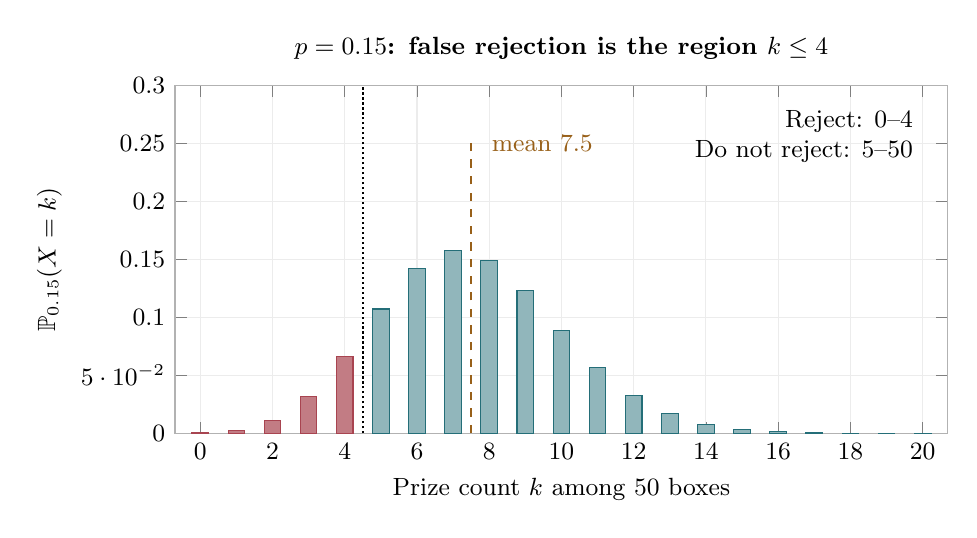
\begin{tikzpicture}
\begin{axis}[
  width=0.94\linewidth,height=6.0cm,
  xmin=-0.7,xmax=20.7,ymin=0,ymax=0.30,
  xtick={0,2,...,20},ytick={0,0.05,...,0.30},
  xlabel={Prize count $k$ among 50 boxes},ylabel={$\Prob_{0.15}(X=k)$},
  title={$p=0.15$: false rejection is the region $k\le4$},
  tick label style={font=\small},label style={font=\small},
  title style={font=\small\bfseries},grid=major,grid style={gray!15},
  axis line style={gray!60}]
\addplot[ybar,bar shift=0pt,bar width=6pt,fill=rose!70,draw=rose] coordinates {
  (0,0.000295764663713) (1,0.00260968820923) (2,0.0112830637281)
  (3,0.0318580622912) (4,0.0660586291627)};
\addplot[ybar,bar shift=0pt,bar width=6pt,fill=teal!50,draw=teal] coordinates {
  (5,0.107248127346) (6,0.1419460509) (7,0.157452762343)
  (8,0.149348576046) (9,0.122992944979) (10,0.0889890131316)
  (11,0.0571052490684) (12,0.0327515399069) (13,0.0168944594995)
  (14,0.00787934875816) (15,0.00333713594463) (16,0.00128823262569)
  (17,0.000454670338477) (18,0.000147099227154)
  (19,4.37198941388e-05) (20,1.19586769262e-05)};
\draw[densely dotted,thick] (axis cs:4.5,0)--(axis cs:4.5,0.30);
\draw[dashed,thick,gold] (axis cs:7.5,0)--(axis cs:7.5,0.255);
\node[font=\small,anchor=west,text=gold] at (axis cs:7.8,0.25) {mean $7.5$};
\node[font=\small,anchor=north east,align=right] at (axis cs:20,0.287)
  {Reject: $0$--$4$\\Do not reject: $5$--$50$};
\end{axis}
\end{tikzpicture}\par
\begin{minipage}{0.94\linewidth}\small
The red bars at $0$--$4$ total $0.1121$. The dotted divider sits between
the two decisions; the dashed gold line marks the mean, derived below.
For readability the plot shows $0$--$20$ on the full support $0$--$50$.
The omitted probability $\Prob_{0.15}(X\ge21)$ is about
$3.90\times10^{-6}$ and belongs to the do-not-reject region.
\end{minipage}
\end{minipage}
\end{center}

\clearpage
\subsection{Cereal example, part (b): missing a false claim at a five-percent rate}
\label{wed-start}

\begin{keyidea}{Wednesday starts here}
Keep the same sample of $50$ boxes and the same rule: reject when $X\le4$.
We now change the assumed true prize rate to $p=0.05$. After evaluating this
second error, we will connect the prize count to a sum of Bernoulli variables
and use that representation to derive its mean and variance.
\end{keyidea}

Now change the assumed truth to $p=0.05$. The sampling rule remains the
same, but $X\sim\Bin(50,0.05)$. The company claim is false, and the error
of interest is \emph{not} rejecting it:
\begin{align*}
\Prob_{0.05}(\text{do not reject})
 &=\Prob_{0.05}(X>4)\\
 &=1-\Prob_{0.05}(X\le4)\\
 &=1-\sum_{k=0}^{4}\binom{50}{k}(0.05)^k(0.95)^{50-k}\\
 &\approx\boxed{0.1036\quad\text{or }10.36\%.}
\end{align*}
Because $X$ is an integer, $X>4$ means $X\ge5$. At a true rate of $5\%$,
this rule misses the false claim about $10.36\%$ of the time.

\begin{center}
\begin{minipage}{\linewidth}
\centering
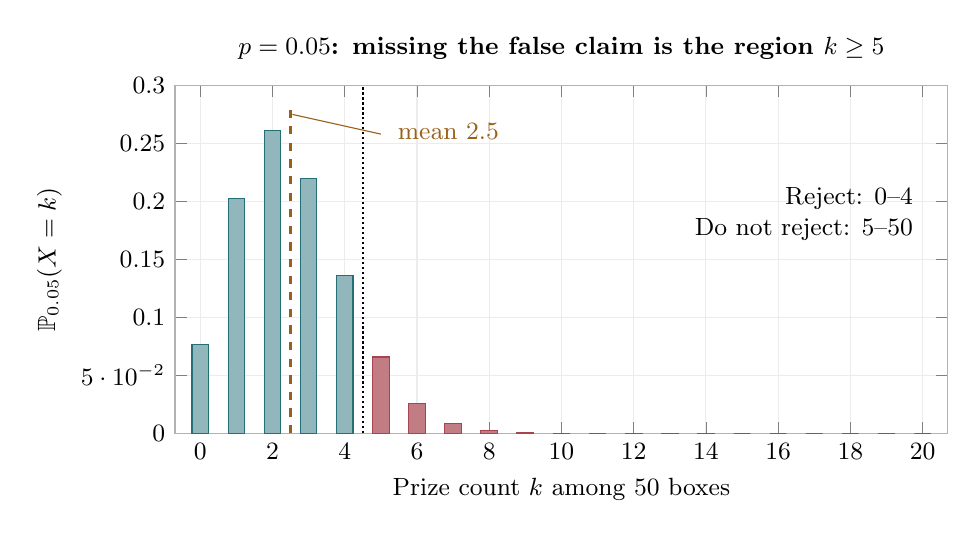
\begin{tikzpicture}
\begin{axis}[
  width=0.94\linewidth,height=6.0cm,
  xmin=-0.7,xmax=20.7,ymin=0,ymax=0.30,
  xtick={0,2,...,20},ytick={0,0.05,...,0.30},
  xlabel={Prize count $k$ among 50 boxes},ylabel={$\Prob_{0.05}(X=k)$},
  title={$p=0.05$: missing the false claim is the region $k\ge5$},
  tick label style={font=\small},label style={font=\small},
  title style={font=\small\bfseries},grid=major,grid style={gray!15},
  axis line style={gray!60}]
\addplot[ybar,bar shift=0pt,bar width=6pt,fill=teal!50,draw=teal] coordinates {
  (0,0.0769449752767) (1,0.202486777044) (2,0.261101370399)
  (3,0.219874838231) (4,0.135975228906)};
\addplot[ybar,bar shift=0pt,bar width=6pt,fill=rose!70,draw=rose] coordinates {
  (5,0.0658406371544) (6,0.0259897251925) (7,0.00859810457497)
  (8,0.00243235853108) (9,0.000597421393598) (10,0.000128917248092)
  (11,2.46731575296e-05) (12,4.2204085248e-06) (13,6.492936192e-07)
  (14,9.03152778586e-08) (15,1.14082456242e-08) (16,1.31344933174e-09)
  (17,1.38257824394e-10) (18,1.3340667266e-11)
  (19,1.18255222303e-12) (20,9.64713655629e-14)};
\draw[densely dotted,thick] (axis cs:4.5,0)--(axis cs:4.5,0.30);
\draw[dashed,thick,gold] (axis cs:2.5,0)--(axis cs:2.5,0.28);
\node[font=\small,anchor=west,text=gold] at (axis cs:5.2,0.26) {mean $2.5$};
\draw[gold,thin] (axis cs:5.0,0.258)--(axis cs:2.55,0.275);
\node[font=\small,anchor=north east,align=right] at (axis cs:20,0.22)
  {Reject: $0$--$4$\\Do not reject: $5$--$50$};
\end{axis}
\end{tikzpicture}\par
\begin{minipage}{0.94\linewidth}\small
The red region now begins at $5$. Its total probability, including the
unplotted counts $21$--$50$, is $0.1036$. The omitted probability is about
$7.79\times10^{-15}$. Both histograms use the same horizontal and vertical
scales so their shapes and decision regions can be compared directly.
\end{minipage}
\end{minipage}
\end{center}

The mean here is $2.5$, but ``above the mean'' is not the same event as
``do not reject.'' Counts $3$ and $4$ are above $2.5$ and still lead to
rejection. The chosen cutoff, not the mean, determines the decision.

\subsection{Two errors, computed under two different truths}

\begin{center}
\begin{tabularx}{\linewidth}{@{}p{0.22\linewidth}L p{0.19\linewidth}@{}}
\toprule
Assumed true rate & Error made by the rule & Probability\\
\midrule
$p=0.15$ & Reject a true claim: $X\le4$ & $0.1121$\\
$p=0.05$ & Do not reject a false claim: $X\ge5$ & $0.1036$\\
\bottomrule
\end{tabularx}
\end{center}
These are different error types under different values of the true
parameter. They are not complementary probabilities, and we do not add
them to obtain one overall error probability without specifying how
often the different true situations arise.

\begin{careful}{What these numbers do and do not answer}
The first number is a probability of a decision \emph{given a true prize
rate}. It is not the probability that the company's claim is true or
false after seeing a sample, nor the probability that a particular
conclusion is wrong. Also, $11.21\%$ alone does not establish that a
sample of $50$ boxes is insufficient. Adequacy depends on the sample
size, the cutoff, the departures we want to detect, and which errors
we are willing to tolerate.
\end{careful}

For example, make rejection harder by changing the cutoff to $X\le3$.
This removes the $X=4$ bar from the rejection region. It reduces false
rejection when the claim is true, but it also adds $X=4$ to the region
where a false claim is missed:
\begin{center}
\begin{tabular}{lcc}
\toprule
Rejection rule & False rejection at $p=0.15$ & Miss at $p=0.05$\\
\midrule
$X\le4$ & $0.1121$ & $0.1036$\\
$X\le3$ & $0.0460$ & $0.2396$\\
\bottomrule
\end{tabular}
\end{center}
The sample size and the cutoff together determine the performance of the
rule. This tradeoff is the intuitive bridge to later work on statistical
testing; the binomial distribution already lets us quantify it.

\section{A binomial count is a sum of Bernoulli variables}
\label{binomial-moments}

For the cereal experiment, define $I_i=1$ when box $i$ contains a prize and
$I_i=0$ otherwise. An outcome such as $(1,0,0,1,0)$ has two prize-bearing
boxes because $1+0+0+1+0=2$. The equality
\[S=I_1+\cdots+I_n\]
is true for every outcome. If the $I_i$ are mutually independent and each
is $\Bernoulli(p)$, any specified sequence with $k$ ones has probability
$p^k(1-p)^{n-k}$. There are $\binom nk$ such disjoint sequences, so
\[\Prob(S=k)=\binom nk p^k(1-p)^{n-k},\qquad S\sim\Bin(n,p).\]
Independence identifies the distribution; the sum representation now gives
us a simpler route to the moments than summing the binomial pmf directly.

\subsection{Mean: add the expectations of the indicators}

Return to the trial indicators. For $S\sim\Bin(n,p)$,
\[
S=X_1+\cdots+X_n,\qquad \E[X_i]=p,\qquad \Var(X_i)=pq.
\]
Instead of directly evaluating the weighted sum
$\sum_{k=0}^{n}k\binom{n}{k}p^kq^{n-k}$, use linearity:
\begin{align*}
\E[S]
 &=\E[X_1+\cdots+X_n]\\
 &=\E[X_1]+\cdots+\E[X_n]\\
 &=\underbrace{p+\cdots+p}_{n\text{ terms}}\\
 &=\boxed{np}.
\end{align*}
This addition of expectations does not require independence. Even if
the trial outcomes were dependent, a sum of $n$ indicators each having
success probability $p$ would still have mean $np$; its distribution
would not necessarily be binomial.

\subsection{Variance: independence removes the cross covariances}

For the binomial model the trial indicators are independent. Therefore
\begin{align*}
\Var(S)
 &=\sum_{i=1}^{n}\Var(X_i)
   +2\sum_{i<j}\Cov(X_i,X_j)\\
 &=\sum_{i=1}^{n}pq+0
 &&\text{independence makes the covariances zero}\\
 &=\boxed{npq=np(1-p)}.
\end{align*}
This is where independence matters in the moment calculation.
Pairwise zero covariance would suffice for the variance identity, but
independence is supplied by our binomial assumptions.

\begin{keyidea}{Binomial moments}
\[
\boxed{S\sim\Bin(n,p)
\quad\Longrightarrow\quad
\E[S]=np,\qquad\Var(S)=np(1-p).}
\]
The mean adds because expectation is linear. The variances add because
the independent indicators have zero cross covariances.
\end{keyidea}

For the two cereal distributions,
\begin{center}
\begin{tabular}{ccc}
\toprule
Distribution & Mean prize count & Variance\\
\midrule
$\Bin(50,0.15)$ & $50(0.15)=7.5$ & $50(0.15)(0.85)=6.375$\\
$\Bin(50,0.05)$ & $50(0.05)=2.5$ & $50(0.05)(0.95)=2.375$\\
\bottomrule
\end{tabular}
\end{center}
A sample cannot contain $7.5$ prize-bearing boxes. The fractional mean
describes the long-run average count across repeated samples of $50$
boxes under the model; it is neither a possible single-sample count nor
a guarantee about the next sample. The variance describes the spread
of those counts around their mean and is measured in squared count units.

\begin{keyidea}{Before changing the sampling model: which addition used independence?}
In $\E[X_1+\cdots+X_n]=\sum_i\E[X_i]$, independence was not needed.
In $\Var(X_1+\cdots+X_n)=\sum_i\Var(X_i)$, we used independence to
remove the covariance terms. More precisely, zero cross covariances
are sufficient. This is the distinction that turns the one-trial
Bernoulli calculations into the binomial mean $np$ and variance $npq$.
\end{keyidea}

% WEDNESDAY CONTINUATION — inlined for a standalone source.
% Student-facing continuation for the cumulative Monday/Wednesday reference.
% Insert after the existing binomial mean and variance section.
% No preamble, external inputs, custom macros, or end-document command.
% Existing macros: \E, \Prob, \Var, \Cov, \Bin; boxes: keyidea and careful.
% Wednesday resumes earlier in the cumulative document at cereal part (b),
% then the existing Bernoulli-sum/binomial-moments material leads here.

\section{A fair coin connects the binomial formula to counting}
\label{fair-coin-start}

We have obtained the binomial model by adding independent Bernoulli
indicators. Its probability formula also connects directly to our earlier
counting methods. Consider $n$ independent flips of a fair coin, and let
$S$ count the heads. Here $p=1/2$, so
\begin{align*}
\Prob(S=k)
 &=\binom nk\left(\frac12\right)^k
          \left(\frac12\right)^{n-k}\\
 &=\boxed{\frac{\binom nk}{2^n}},
 \qquad k=0,1,\ldots,n.
\end{align*}
The two exponents add to $n$. Every complete sequence of $n$ flips has
probability $1/2^n$, and there are $2^n$ possible sequences.
Exactly $\binom nk$ of them place heads in $k$ positions.

\subsection{Four flips: count the sequences with two heads}

The six favorable sequences are
\[
\mathrm{HHTT},\quad \mathrm{HTHT},\quad \mathrm{HTTH},\quad
\mathrm{THHT},\quad \mathrm{THTH},\quad \mathrm{TTHH}.
\]
There are $2^4=16$ equally likely sequences altogether. Therefore,
\[
\Prob(S=2)=\frac{6}{16}=\frac38.
\]
This is the same answer obtained from
$\binom42(1/2)^2(1/2)^2$. The binomial coefficient counts the favorable
sequences; the factors of $1/2$ assign their probabilities.

\begin{keyidea}{When does favorable divided by total apply?}
For independent fair flips, all $2^n$ complete sequences are equally
likely, so counting favorable sequences and dividing by $2^n$ works.
For an independent biased coin, a sequence with $k$ heads still has
probability $p^k(1-p)^{n-k}$, but sequences with different numbers of heads
need not be equally likely. Keep the probability weights in that case.
\end{keyidea}

\textbf{Check.} Why is $\Prob(S=k)=\binom nk/2^n$ a special case?
It uses both independence of the flips and $p=1/2$. Equal probabilities
of heads and tails on each individual trial alone do not establish
independence across trials.

\section{Replacement connects the counting models}
\label{replacement-start}

Now replace the coin with a finite collection of $N$ distinct objects.
Exactly $K$ objects are labeled a success, and the other $N-K$ are labeled
a failure. Draw $n$ times. Let $X$ be the number of successes drawn.
The sampling procedure determines the distribution of $X$.

\subsection{With replacement: the same composition on every draw}

Suppose we select one of the $N$ objects uniformly, record its label,
replace it, and independently select again. Each draw has success
probability
\[
p=\frac KN.
\]
Replacing the selected object restores the same collection. The
independent uniform selections give independent Bernoulli trials, so
\[
X\sim\Bin\left(n,\frac KN\right).
\]
There is a counting route to the same answer. With order recorded and
replacement allowed, there are $N^n$ equally likely object sequences.
For a sequence with exactly $k$ successes:
\begin{enumerate}
\item Choose the $k$ success positions: $\binom nk$ choices.
\item Fill those positions using the $K$ successful objects:
$K^k$ choices.
\item Fill the remaining positions using the $N-K$ unsuccessful objects:
$(N-K)^{n-k}$ choices.
\end{enumerate}
Thus
\begin{align*}
\Prob(X=k)
 &=\frac{\binom nk K^k(N-K)^{n-k}}{N^n}\\
 &=\binom nk\left(\frac KN\right)^k
              \left(1-\frac KN\right)^{n-k}.
\end{align*}
This is exactly the binomial formula. Replacement and independent
selection allow the same object to appear more than once in the
recorded sequence.

\subsection{Without replacement: the remaining collection changes}

If we keep each selected object out of the collection, an observed success
changes what remains. For $0<K<N$ and $N>1$,
\[
\Prob(\text{first draw is a success})=\frac KN,
\]
whereas
\[
\Prob(\text{second success}\mid\text{first success})
 =\frac{K-1}{N-1}<\frac KN.
\]
After a failure instead,
\[
\Prob(\text{second success}\mid\text{first failure})
 =\frac K{N-1}>\frac KN.
\]
The label on the first draw therefore gives information about the next
draw. The draw indicators are dependent, even though each draw position
has the same success probability $K/N$ before any outcomes are observed.
We need a distribution that accounts for this sampling procedure.

\section{The hypergeometric distribution: a count without replacement}
\label{hypergeometric-start}

\begin{keyidea}{Label the population and the sample separately}
\begin{center}
\begin{tabular}{cl}
\toprule
Symbol & Meaning\\
\midrule
$N$ & Total number of objects in the population\\
$K$ & Number of successes in the population\\
$n$ & Number of objects in the sample\\
$k$ & A possible number of successes in that sample\\
\bottomrule
\end{tabular}
\end{center}
The population has $K$ successes and $N-K$ failures. A sample containing
$k$ successes contains $n-k$ failures. Here $N\ge1$,
$0\le K\le N$, and $0\le n\le N$, all integers.
\end{keyidea}

Assume a \emph{simple random sample without replacement}: every subset
of $n$ distinct population objects is equally likely. There are
$\binom Nn$ such samples.

To obtain exactly $k$ successes, select $k$ of the $K$ successful objects
and $n-k$ of the $N-K$ unsuccessful objects. Once those two selections
are made, the sample is determined. Hence
\[
\boxed{\Prob(X=k)
 =\frac{\binom Kk\binom{N-K}{n-k}}{\binom Nn}.}
\]
We write
\[
X\sim\operatorname{Hypergeometric}(N,K,n).
\]
The numerator counts the favorable samples. The denominator counts all
equally likely samples. Both counts treat the sample as an unordered
set of distinct objects.

\subsection{Which values of the count are possible?}

We cannot draw a negative number of successes or more than the $K$
successes available. We also cannot draw more successes than the sample
size $n$. Finally, if the population has only $N-K$ failures, a sample
of size $n$ must contain at least $n-(N-K)$ successes whenever that
quantity is positive. Combining these restrictions gives
\[
\boxed{\max(0,n+K-N)\le k\le\min(n,K).}
\]
Outside this integer range the probability is zero.

\textbf{Check.} A population has $N=10$ objects, of which $K=8$ are
successes. We draw $n=5$ without replacement. The smallest possible
success count is three, because only two failures exist. The largest
is five. Thus the support is $\{3,4,5\}$.

\subsection{Why the probabilities sum to one}

Every sample has exactly one possible success count. Grouping all
$n$-element samples by that count gives
\[
\sum_k\binom Kk\binom{N-K}{n-k}=\binom Nn,
\]
where the sum runs over feasible $k$. Dividing by $\binom Nn$ gives
$\sum_k\Prob(X=k)=1$. This is a counting proof of the normalization:
the groups partition the set of all possible samples.

\subsection{A balanced population is still different from independent fair flips}

Take $N=10$, $K=5$, and $n=4$. Each draw position has marginal success
probability $1/2$. Without replacement,
\[
\Prob(X=2)=\frac{\binom52\binom52}{\binom{10}4}
 =\frac{100}{210}=\frac{10}{21}\approx0.47619.
\]
The independent fair-coin probability was $3/8=0.375$.
Both experiments have success probability $1/2$ at each position, but
their joint behavior differs. The without-replacement sample is more
concentrated around its mean of two in this example.

\subsection{Source example: how many purple candies?}

A bag contains $50$ candies of each of five colors, for $250$ candies
altogether. Select $12$ uniformly without replacement. A success is
selecting a purple candy. Therefore
\[
N=250,\qquad K=50,\qquad n=12.
\]
Exactly half the sample being purple means $X=6$, so
\[
\Prob(X=6)
 =\frac{\binom{50}6\binom{200}6}{\binom{250}{12}}
 \approx0.0137602.
\]
The second factor chooses six nonpurple candies, because a sample of
twelve with six purple candies must have six of the other colors.
We group all nonpurple colors together as failures.

\section{Hypergeometric moments from the same indicator strategy}
\label{hypergeometric-moments}

The count still has an indicator representation. Imagine the uniform
sample being drawn sequentially without replacement, and define
\[
I_i=
\begin{cases}
1,&\text{draw }i\text{ is a success},\\
0,&\text{draw }i\text{ is a failure}.
\end{cases}
\qquad X=I_1+\cdots+I_n.
\]
The indicators are dependent. We will retain the covariance terms
instead of discarding them.

\subsection{Mean: the marginal chance at each position is still $K/N$}

Before any draws are observed, each of the $N$ objects is equally likely
to occupy a particular draw position. Exactly $K$ objects are successes,
so
\[
\Prob(I_i=1)=\frac KN=:p
\quad\text{for every }i.
\]
This is a marginal probability. It does not say the conditional chance
stays fixed after earlier results are revealed.

By linearity,
\begin{align*}
\E[X]
 &=\E[I_1]+\cdots+\E[I_n]\\
 &=\frac KN+\cdots+\frac KN\\
 &=\boxed{n\frac KN=np}.
\end{align*}
The mean agrees with the binomial mean for the same $n$ and $p$.
The derivation remains valid because linearity never required
independence.

\subsection{Covariance: two successes compete for the finite supply}

Assume $N>1$. For two different draw positions $i$ and $j$, the product
$I_iI_j$ is one exactly when both positions contain successes.
Uniform sampling without replacement gives
\[
\E[I_iI_j]
 =\Prob(I_i=1,I_j=1)
 =\frac KN\frac{K-1}{N-1}.
\]
When $K=0$, the joint probability is zero directly; the displayed product
has that same value. For $K>0$, the second factor is the conditional
chance after one success is used.

Use the covariance identity and put both terms over a common denominator:
\begin{align*}
\Cov(I_i,I_j)
 &=\E[I_iI_j]-\E[I_i]\E[I_j]\\
 &=\frac{K(K-1)}{N(N-1)}-\frac{K^2}{N^2}\\
 &=\frac{NK(K-1)-K^2(N-1)}{N^2(N-1)}\\
 &=-\frac{K(N-K)}{N^2(N-1)}\\
 &=-\frac{p(1-p)}{N-1}.
\end{align*}
For $0<K<N$, this covariance is negative. A success at one position
leaves fewer successes available for another.

\subsection{Variance: add the covariance contributions}

Each $I_i$ is marginally Bernoulli$(p)$, so
$\Var(I_i)=p(1-p)$. There are $\binom n2$ distinct unordered pairs
of positions. Therefore
\begin{align*}
\Var(X)
 &=\sum_{i=1}^{n}\Var(I_i)
   +2\sum_{i<j}\Cov(I_i,I_j)\\
 &=np(1-p)
   +2\binom n2\left(-\frac{p(1-p)}{N-1}\right)\\
 &=np(1-p)-\frac{n(n-1)p(1-p)}{N-1}\\
 &=np(1-p)\left(1-\frac{n-1}{N-1}\right)\\
 &=\boxed{np(1-p)\frac{N-n}{N-1}}.
\end{align*}

\begin{keyidea}{Hypergeometric mean and variance}
For $X\sim\operatorname{Hypergeometric}(N,K,n)$, set $p=K/N$.
Then
\[
\E[X]=np,\qquad
\Var(X)=np(1-p)\underbrace{\frac{N-n}{N-1}}_
 {\text{finite-population correction}}\quad(N>1).
\]
The mean uses linearity. The variance records the negative covariances
created by sampling without replacement.
\end{keyidea}

The correction provides useful checks:
\begin{itemize}
\item If $n=1$, the correction is one. A single draw is Bernoulli$(p)$.
\item If $n=N$, the correction is zero. Inspecting the entire population
gives exactly $K$ successes, with no uncertainty in the count.
\item If $n$ is small relative to $N$, the correction is close to one,
so the variance is close to the binomial variance.
\end{itemize}
If $N=1$, handle the sample directly: the only possible sample sizes
are zero and one, and its success count is fixed by the population.
The formula with denominator $N-1$ is not used in that case.

For the candy example,
\[
\E[X]=12\left(\frac{50}{250}\right)=2.4,
\]
and
\[
\Var(X)
 =12(0.2)(0.8)\frac{250-12}{250-1}
 =1.92\frac{238}{249}
 \approx1.83518.
\]
Independent sampling with replacement would have the same mean $2.4$
and variance $1.92$. Sampling without replacement reduces the variance.

\section{Why hypergeometric counts approach binomial counts}
\label{hypergeometric-limit}

Keep the sample size $n$ fixed while the population becomes larger.
If we remove only a few objects from a very large population, each
removal makes a small change in the remaining success proportion.
This suggests that sampling without replacement should resemble
independent sampling with replacement.

Make the statement precise. Let $N$ grow, allow $K=K_N$ to grow with it,
and suppose
\[
n\text{ is fixed},\qquad
N\longrightarrow\infty,\qquad
\frac{K_N}{N}\longrightarrow p,\qquad 0<p<1.
\]
In particular, both the number of successes and the number of failures
grow without bound. If
$X_N\sim\operatorname{Hypergeometric}(N,K_N,n)$, then
\[
\boxed{\Prob(X_N=k)\longrightarrow
\binom nk p^k(1-p)^{n-k}
\quad\text{for each }k=0,1,\ldots,n.}
\]
Thus the distribution approaches $\Bin(n,p)$.

\subsection{Derive the limit directly from the counting formula}

Write $a_{\underline r}=a(a-1)\cdots(a-r+1)$ for the falling factorial,
with $a_{\underline0}=1$. Expanding the binomial coefficients gives
\[
\frac{\binom Kk\binom{N-K}{n-k}}{\binom Nn}
 =\binom nk\frac{K_{\underline k}(N-K)_{\underline{n-k}}}
                    {N_{\underline n}}.
\]
For $K=K_N$, divide numerator and denominator by $N^n$:
\[
\Prob(X_N=k)
=\binom nk
\frac{
 \displaystyle\prod_{j=0}^{k-1}\left(\frac{K_N}{N}-\frac jN\right)
 \displaystyle\prod_{j=0}^{n-k-1}
       \left(1-\frac{K_N}{N}-\frac jN\right)}
 {\displaystyle\prod_{j=0}^{n-1}\left(1-\frac jN\right)}.
\]
An empty product equals one. Since $n$ and $k$ stay fixed, only finitely
many factors appear. In the limit the first product becomes $p^k$,
the second becomes $(1-p)^{n-k}$, and the denominator becomes one.
That proves the displayed binomial limit.

The moments agree with this picture:
\[
\E[X_N]=n\frac{K_N}{N}\longrightarrow np,
\]
\[
\Var(X_N)
 =n\frac{K_N}{N}\left(1-\frac{K_N}{N}\right)
   \frac{N-n}{N-1}
 \longrightarrow np(1-p).
\]
The correction tends to one because $n$ is fixed while $N$ increases.

\label{simulation-start}
% Generated by simulate-hypergeometric.py. Do not edit numerical data by hand.
% Fragment only: requires amsmath, xcolor, and PGFPlots compat=1.18.
% No groupplots library, external images, data files, or shell escape required.
% Each panel is unbreakable; page breaks are allowed between panels.
\begingroup
\noindent\textbf{A fixed sample from a growing population.}
Keep the sample size $n=10$ and success fraction $p=K/N=1/2$ fixed.
Increase the population through $N=12,40,400$, with $K=N/2$ successes.
Sampling is without replacement within each sample; the population is reset
before the next Monte Carlo repetition.

\smallskip
\noindent Blue bars are the \textbf{exact hypergeometric probabilities}.
Orange open diamonds are the \textbf{exact $\operatorname{Bin}(10,1/2)$ probabilities}.
Black crosses are \textbf{Monte Carlo relative frequencies} from $100{,}000$
repetitions per panel. Marks refer only to integer counts, not a density.
All panels have the same axes, show every count $k=0,\ldots,10$, and omit no mass.

\par\medskip
\noindent\begin{minipage}{\linewidth}
\centering
{\small\bfseries Population $N=12$, with $K=6$ successes; sample $n=10$}\par
{\small Sample fraction $n/N=83.33\%$; exact support $\{4,5,6\}$; exact variance $0.454545$}\par
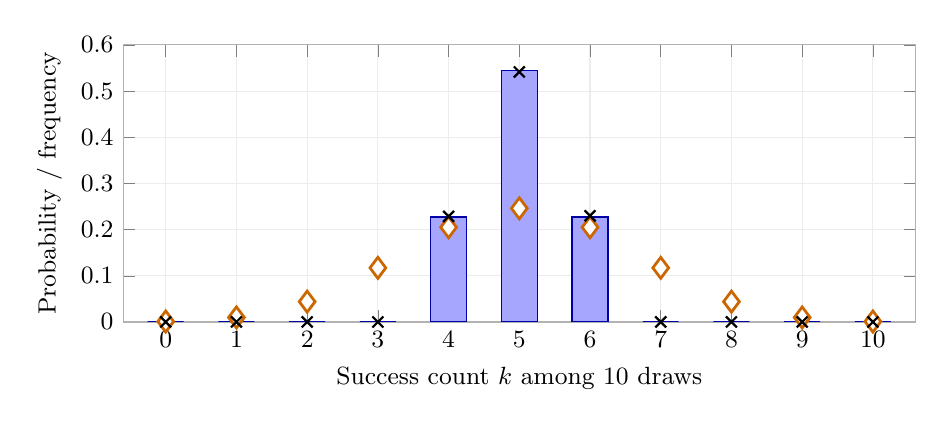
\begin{tikzpicture}
\begin{axis}[
  width=0.96\linewidth,height=5.1cm,
  xmin=-0.6,xmax=10.6,ymin=0,ymax=0.60,
  xtick={0,1,...,10},ytick={0,0.1,...,0.6},
  xlabel={Success count $k$ among $10$ draws},ylabel={Probability / frequency},
  tick label style={font=\small},label style={font=\small},
  scaled y ticks=false,grid=major,grid style={gray!15},
  axis line style={gray!60}]
\addplot[ybar,bar shift=0pt,bar width=13pt,
  fill=blue!35,draw=blue!65!black] coordinates {
  (0,0)
  (1,0)
  (2,0)
  (3,0)
  (4,0.22727272727273)
  (5,0.54545454545455)
  (6,0.22727272727273)
  (7,0)
  (8,0)
  (9,0)
  (10,0)
};
\addplot[only marks,mark=diamond*,mark size=3.8pt,
  color=orange!80!black,mark options={fill=white,line width=1pt}] coordinates {
  (0,0.0009765625)
  (1,0.009765625)
  (2,0.0439453125)
  (3,0.1171875)
  (4,0.205078125)
  (5,0.24609375)
  (6,0.205078125)
  (7,0.1171875)
  (8,0.0439453125)
  (9,0.009765625)
  (10,0.0009765625)
};
\addplot[only marks,mark=x,mark size=2.8pt,
  color=black,mark options={line width=0.8pt}] coordinates {
  (0,0)
  (1,0)
  (2,0)
  (3,0)
  (4,0.2286)
  (5,0.54144)
  (6,0.22996)
  (7,0)
  (8,0)
  (9,0)
  (10,0)
};
\end{axis}
\end{tikzpicture}
\end{minipage}

\par\medskip
\noindent\begin{minipage}{\linewidth}
\centering
{\small\bfseries Population $N=40$, with $K=20$ successes; sample $n=10$}\par
{\small Sample fraction $n/N=25.00\%$; exact support $\{0,1,\ldots,10\}$; exact variance $1.923077$}\par
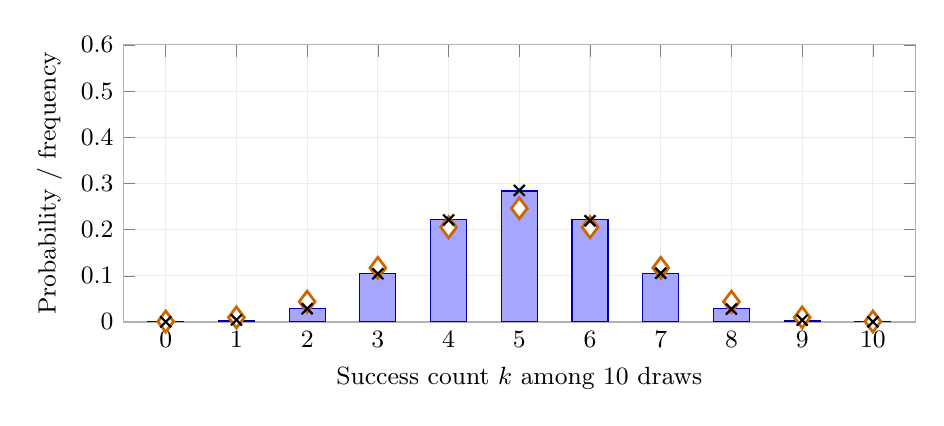
\begin{tikzpicture}
\begin{axis}[
  width=0.96\linewidth,height=5.1cm,
  xmin=-0.6,xmax=10.6,ymin=0,ymax=0.60,
  xtick={0,1,...,10},ytick={0,0.1,...,0.6},
  xlabel={Success count $k$ among $10$ draws},ylabel={Probability / frequency},
  tick label style={font=\small},label style={font=\small},
  scaled y ticks=false,grid=major,grid style={gray!15},
  axis line style={gray!60}]
\addplot[ybar,bar shift=0pt,bar width=13pt,
  fill=blue!35,draw=blue!65!black] coordinates {
  (0,0.00021795989537925)
  (1,0.0039629071887136)
  (2,0.028235713719585)
  (3,0.10425494296462)
  (4,0.22154175379982)
  (5,0.28357344486377)
  (6,0.22154175379982)
  (7,0.10425494296462)
  (8,0.028235713719585)
  (9,0.0039629071887136)
  (10,0.00021795989537925)
};
\addplot[only marks,mark=diamond*,mark size=3.8pt,
  color=orange!80!black,mark options={fill=white,line width=1pt}] coordinates {
  (0,0.0009765625)
  (1,0.009765625)
  (2,0.0439453125)
  (3,0.1171875)
  (4,0.205078125)
  (5,0.24609375)
  (6,0.205078125)
  (7,0.1171875)
  (8,0.0439453125)
  (9,0.009765625)
  (10,0.0009765625)
};
\addplot[only marks,mark=x,mark size=2.8pt,
  color=black,mark options={line width=0.8pt}] coordinates {
  (0,0.00022)
  (1,0.0043)
  (2,0.02866)
  (3,0.10432)
  (4,0.22084)
  (5,0.28487)
  (6,0.21916)
  (7,0.10557)
  (8,0.02791)
  (9,0.00384)
  (10,0.00031)
};
\end{axis}
\end{tikzpicture}
\end{minipage}

\par\medskip
\noindent\begin{minipage}{\linewidth}
\centering
{\small\bfseries Population $N=400$, with $K=200$ successes; sample $n=10$}\par
{\small Sample fraction $n/N=2.50\%$; exact support $\{0,1,\ldots,10\}$; exact variance $2.443609$}\par
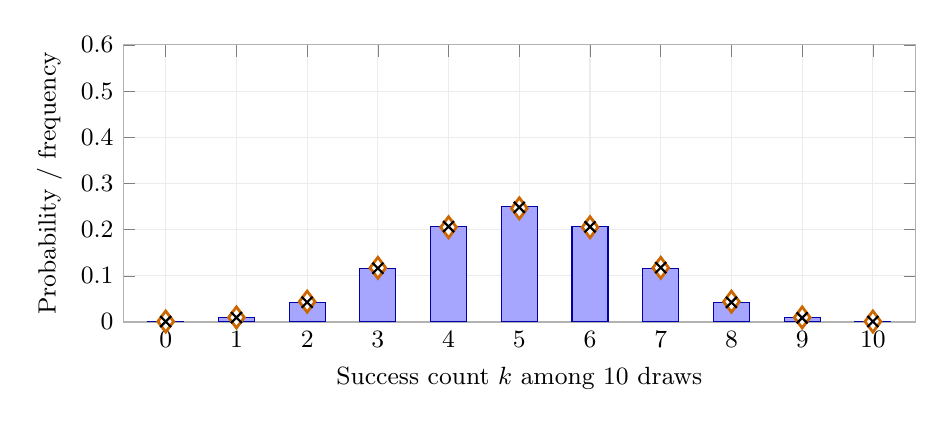
\begin{tikzpicture}
\begin{axis}[
  width=0.96\linewidth,height=5.1cm,
  xmin=-0.6,xmax=10.6,ymin=0,ymax=0.60,
  xtick={0,1,...,10},ytick={0,0.1,...,0.6},
  xlabel={Success count $k$ among $10$ draws},ylabel={Probability / frequency},
  tick label style={font=\small},label style={font=\small},
  scaled y ticks=false,grid=major,grid style={gray!15},
  axis line style={gray!60}]
\addplot[ybar,bar shift=0pt,bar width=13pt,
  fill=blue!35,draw=blue!65!black] coordinates {
  (0,0.00087025887724498)
  (1,0.009112658400471)
  (2,0.042502008320947)
  (3,0.11627492431844)
  (4,0.20662773277724)
  (5,0.24922483461131)
  (6,0.20662773277724)
  (7,0.11627492431844)
  (8,0.042502008320947)
  (9,0.009112658400471)
  (10,0.00087025887724498)
};
\addplot[only marks,mark=diamond*,mark size=3.8pt,
  color=orange!80!black,mark options={fill=white,line width=1pt}] coordinates {
  (0,0.0009765625)
  (1,0.009765625)
  (2,0.0439453125)
  (3,0.1171875)
  (4,0.205078125)
  (5,0.24609375)
  (6,0.205078125)
  (7,0.1171875)
  (8,0.0439453125)
  (9,0.009765625)
  (10,0.0009765625)
};
\addplot[only marks,mark=x,mark size=2.8pt,
  color=black,mark options={line width=0.8pt}] coordinates {
  (0,0.00085)
  (1,0.00948)
  (2,0.0427)
  (3,0.11634)
  (4,0.20655)
  (5,0.24818)
  (6,0.20599)
  (7,0.11759)
  (8,0.04252)
  (9,0.00882)
  (10,0.00098)
};
\end{axis}
\end{tikzpicture}
\end{minipage}

\par\medskip
\noindent\textbf{Measure the difference using exact probabilities.}
The common mean is $np=5$. Sampling without replacement reduces the variance:
\[
 \operatorname{Var}(X_N)=np(1-p)\frac{N-n}{N-1}
 =2.5\frac{N-10}{N-1}\longrightarrow 2.5.
\]
The total variation distance compares the two complete probability tables:
\[
 d_{\mathrm{TV}}(X_N,B)=\frac12\sum_{k=0}^{10}
 \left|\Pr(X_N=k)-\Pr(B=k)\right|,
 \qquad B\sim\operatorname{Bin}(10,1/2).
\]
It is the largest difference in probability the two models assign to the
same event. Here it is calculated from exact formulas, not simulated counts.

\begin{center}
\small
\begin{tabular}{rrrrr}
\hline
$N$ & $K$ & Sample fraction $n/N$ & Exact variance & Exact $d_{\mathrm{TV}}$\\
\hline
12 & 6 & 83.33\% & 0.454545 & 0.343750\\
40 & 20 & 25.00\% & 1.923077 & 0.070407\\
400 & 200 & 2.50\% & 2.443609 & 0.006230\\
\hline
\multicolumn{3}{l}{Binomial limit, $n=10$, $p=1/2$} & $2.500000$ & $0$\\
\hline
\end{tabular}
\end{center}

\noindent\small\textbf{How to read the comparison.}
For $N=12$, drawing $10$ of the $12$ objects forces the count into $4,5,6$.
The binomial model still assigns mass to $0,\ldots,10$, so it is a poor
approximation. As $N$ grows with $n$ fixed, the sample fraction becomes small,
the variance approaches $2.5$, and the exact bars approach the orange marks.
We are keeping $n$ fixed: this is a binomial limit, not a normal approximation.

\noindent\small\textbf{Simulation illustrates; it does not prove convergence.}
The three populations use seeds $20260942$, $20260970$, and $20261330$
(base seed $20260930$ plus $N$), with $100{,}000$ repetitions each.
The black crosses fluctuate around the exact blue bars. In the last panel,
sampling noise can obscure the small remaining difference from the binomial
model. The limit requires the mathematical PMF argument; neither a simulation
nor three finite comparisons prove it.
\endgroup


\subsection{What to look for in the comparison}

Compare the probabilities assigned to each possible count $k$, keeping
the sample size and limiting success proportion fixed. As the population
grows, the hypergeometric probabilities should approach the binomial
probabilities at every count. The smaller population has a more
concentrated distribution because a larger fraction of it is sampled.

If a figure includes simulated frequencies, each repetition must start
from the full original population, take a fresh sample without
replacement, and record the success count. Across many repetitions,
the relative frequencies estimate the hypergeometric pmf. Their random
fluctuations are simulation noise; the exact pmf gives the underlying
distribution to which those frequencies are compared.

\begin{careful}{Keep the sample size fixed in this limit}
The statement above fixes $n$. Merely making $N$ large does not make
dependence negligible if the sample also occupies a substantial fraction
of the population. The ratio $(N-n)/(N-1)$ makes this distinction visible.
For example, sampling half the population retains a correction near
$1/2$ rather than near one.
\end{careful}

\section{Poisson begins with a concrete rare-event count}
\label{poisson-example}

Suppose a laboratory processes $1000$ specimens. Under a simplified
model, each specimen independently experiences a particular rare
processing error with probability $0.002$. Let $X$ count the specimens
with that error.

The exact count model is
\[
X\sim\Bin(1000,0.002).
\]
Although there are many opportunities, the error probability at each
opportunity is small. The expected number of errors is
\[
\E[X]=1000(0.002)=2.
\]
We can already answer concrete probability questions using the binomial
formula:
\begin{align*}
\Prob(X=0)
 &=(0.998)^{1000}\approx0.135065,\\
\Prob(X\ge1)
 &=1-(0.998)^{1000}\approx0.864935,\\
\Prob(X=2)
 &=\binom{1000}{2}(0.002)^2(0.998)^{998}
 \approx0.270942.
\end{align*}
The variance is $1000(0.002)(0.998)=1.996$, which is close to the mean
of two.

Now imagine more opportunities, each with a smaller error probability,
while keeping the expected total at two. For example, $2000$ independent
opportunities with probability $0.001$ again have expected count two.
This is the setting behind the Poisson approximation: many small,
independent chances combine into a count with a moderate expected value.

\begin{keyidea}{The parameter records the expected total}
For a rare-event binomial approximation, set
\[
\lambda=np.
\]
The laboratory example has $\lambda=2$. The parameter describes the
expected number of events in the entire specified collection of
opportunities.
\end{keyidea}

\section{The Poisson probability mass function}
\label{poisson-start}

A Poisson random variable with parameter $\lambda>0$ has pmf
\[
\boxed{\Prob(Y=k)=e^{-\lambda}\frac{\lambda^k}{k!},
\qquad k=0,1,2,\ldots.}
\]
We write $Y\sim\operatorname{Poisson}(\lambda)$. This distribution gives
probabilities to nonnegative integer counts. Its support has no finite
upper bound.

For the laboratory example, use $Y\sim\operatorname{Poisson}(2)$.
The resulting approximations are
\begin{align*}
\Prob(X=0)&\approx\Prob(Y=0)=e^{-2}\approx0.135335,\\
\Prob(X\ge1)&\approx1-e^{-2}\approx0.864665,\\
\Prob(X=2)&\approx e^{-2}\frac{2^2}{2!}\approx0.270671.
\end{align*}
Compare these with the exact binomial values above. The approximation
is close for these probabilities. It replaces the separate parameters
$n$ and $p$ with their product $\lambda=np$.

\begin{careful}{Approximation and exact model are different statements}
The laboratory model is exactly binomial under the assumptions stated.
Poisson provides an approximation here. A Poisson variable can exceed
$1000$, whereas the binomial count cannot; in this example the Poisson
probability of such counts is extremely small. Keep the exact model
and the approximation distinct.
\end{careful}

\subsection{Why do the Poisson probabilities sum to one?}

Recall the exponential series:
\[
e^\lambda=\sum_{k=0}^{\infty}\frac{\lambda^k}{k!}.
\]
All the Poisson probabilities are nonnegative, and
\begin{align*}
\sum_{k=0}^{\infty}\Prob(Y=k)
 &=e^{-\lambda}\sum_{k=0}^{\infty}\frac{\lambda^k}{k!}\\
 &=e^{-\lambda}e^\lambda\\
 &=1.
\end{align*}
Thus the formula defines a valid pmf. Also $0!=1$, so the zero-count
probability is simply $\Prob(Y=0)=e^{-\lambda}$.
The case $\lambda=0$ can be included separately as the deterministic
count $Y=0$.

\section{Derive Poisson as a limit of binomial distributions}
\label{poisson-limit}

Fix $\lambda>0$. For each sufficiently large integer $m$, consider
\[
Y_m\sim\Bin\left(m,\frac{\lambda}{m}\right).
\]
The number of trials is $m$, the success chance is $\lambda/m$, and
the expected count is always $\lambda$. We use $m$ here to emphasize
that this number of opportunities is changing.

For a fixed count $k$ and sufficiently large $m$,
\[
\Prob(Y_m=k)
 =\binom mk\left(\frac{\lambda}{m}\right)^k
   \left(1-\frac{\lambda}{m}\right)^{m-k}.
\]
Rearrange the factors:
\begin{align*}
\Prob(Y_m=k)
 &=
 \frac{m(m-1)\cdots(m-k+1)}{m^k}
 \frac{\lambda^k}{k!}\\
 &\hspace{1.2em}\cdot
 \left(1-\frac{\lambda}{m}\right)^m
 \left(1-\frac{\lambda}{m}\right)^{-k}.
\end{align*}
Each of the $k$ ratios in the first factor approaches one. The standard
exponential limit gives
\[
\left(1-\frac{\lambda}{m}\right)^m\longrightarrow e^{-\lambda},
\]
and the final factor approaches one because $k$ is fixed. Hence
\[
\boxed{\Prob(Y_m=k)\longrightarrow
 e^{-\lambda}\frac{\lambda^k}{k!}.}
\]
For $k=0$, the empty product in the first factor is one.

More generally, if $m\to\infty$ and $mp_m\to\lambda>0$, then
$p_m\to0$ and $\Bin(m,p_m)$ approaches
$\operatorname{Poisson}(\lambda)$. One can see the same limit by replacing
$\lambda$ in the calculation above with $mp_m$:
$(mp_m)^k\to\lambda^k$ and
$m\log(1-p_m)\to-\lambda$.

\subsection{Compare a source example numerically}

For the source's parameters $m=100$ and $p=0.05$, use $\lambda=5$.
\begin{center}
\begin{tabular}{ccc}
\toprule
$k$ & Exact $\Bin(100,0.05)$ probability
    & $\operatorname{Poisson}(5)$ probability\\
\midrule
0 & 0.00592 & 0.00674\\
1 & 0.03116 & 0.03369\\
2 & 0.08118 & 0.08422\\
3 & 0.13958 & 0.14037\\
4 & 0.17814 & 0.17547\\
\bottomrule
\end{tabular}
\end{center}
The expected count is five in both models. The quality of the
approximation depends on the parameters and the probability being
estimated. There is no need to approximate when an exact binomial
calculation is convenient.

\section{Poisson counts over time, area, or volume}
\label{poisson-exposure}

The rare-opportunity picture also motivates a model for events over a
fixed exposure. Suppose a detector records events at a constant rate
$r$ per minute. For an observation lasting $t$ minutes, define
\[
\lambda=rt.
\]
The rate $r$ has units of events per minute. The parameter $\lambda$
is the expected number of events in this particular window.

\subsection{State the assumptions before assigning the model}

A homogeneous Poisson model for event times uses these properties:
\begin{itemize}
\item Counts in disjoint time intervals are independent.
\item The rate $r$ stays constant throughout the observation.
\item Over a very short interval of length $h$, the probability of
one event is approximately $rh$, while the probability of two or more
events is negligible compared with $h$.
\end{itemize}
Under these assumptions, the count in a window of length $t$ is
$\operatorname{Poisson}(rt)$.

To connect this to the binomial construction, divide the \emph{same}
window into $m$ short pieces. Each piece has duration $t/m$ and
approximately $rt/m=\lambda/m$ chance of an event.
The number of pieces containing an event is approximately
$\Bin(m,\lambda/m)$. Refining the pieces makes multiple events in
a single piece negligible, so the occupied-piece count approaches
the event count. The observation window stays fixed throughout.

\begin{keyidea}{Refining the pieces does not extend the observation}
More pieces means more opportunities with a smaller chance per
opportunity. The total expected count remains
$m(\lambda/m)=\lambda$. Increasing $m$ with a fixed positive success
probability instead would make the expected count grow without bound.
\end{keyidea}

\subsection{A worked example with changing exposure}

Suppose the detector model is appropriate with rate $r=3$ events per
minute. For the count $Z$ in one minute, $\lambda=3$:
\[
\Prob(Z=2)=e^{-3}\frac{3^2}{2!}\approx0.224042,
\]
\[
\Prob(Z\ge1)=1-\Prob(Z=0)=1-e^{-3}\approx0.950213.
\]
For a $30$-second observation, first convert the duration to
$t=0.5$ minute. The count $W$ then has parameter $\lambda=3(0.5)=1.5$,
so
\[
\Prob(W\ge1)=1-e^{-1.5}\approx0.776870.
\]
For two minutes the parameter is six. Changing the window changes
the count distribution even though the event rate remains three per
minute.

\subsection{Read the source's examples as models with assumptions}

The source uses an amoeba reproduction illustration. Its mathematical
point is an idealized source generating events over a fixed interval
$[t_0,t]$ with a constant rate and independent increments. Under the
small-interval condition above, the count has parameter $r(t-t_0)$.
This is an event-source model, not a literal claim that one amoeba
repeatedly survives binary fission. Counting events from a growing
collection of descendants would require reassessing the rate and
independence assumptions.

The same exposure idea applies to the other source illustrations:
\begin{itemize}
\item \textbf{Raindrops:} count drops striking a specified area during
a specified interval. With a homogeneous rate per unit area per unit
time, multiply that rate by the area and duration.
\item \textbf{Price jumps:} define what qualifies as one jump and count
such events during a specified week. A constant-rate Poisson model
also requires independent counts over disjoint intervals; a shared
trigger or clustering can make that assumption unsuitable.
\item \textbf{Stars:} count objects inside a fixed volume. With
homogeneous spatial intensity $\rho$, the parameter is $\lambda=\rho V$.
For the source's $500$ cubic light-years, it is $500\rho$.
Independent counts in disjoint regions are part of the model.
\end{itemize}
These settings suggest potential applications. They do not by
themselves establish the constant-intensity and independence assumptions.

\section{Poisson expectation and variance}
\label{poisson-moments}

The binomial limit suggests the answer. For
$Y_m\sim\Bin(m,\lambda/m)$,
\[
\E[Y_m]=\lambda,\qquad
\Var(Y_m)=\lambda\left(1-\frac{\lambda}{m}\right)
\longrightarrow\lambda.
\]
This motivates the Poisson moment formulas. We now verify them
directly from the pmf.

\subsection{Expectation: cancel one factor and reindex}

Let $Y\sim\operatorname{Poisson}(\lambda)$. Then
\begin{align*}
\E[Y]
 &=\sum_{k=0}^{\infty}k e^{-\lambda}\frac{\lambda^k}{k!}\\
 &=e^{-\lambda}\sum_{k=1}^{\infty}
       \frac{\lambda^k}{(k-1)!}\\
 &=\lambda e^{-\lambda}\sum_{k=1}^{\infty}
       \frac{\lambda^{k-1}}{(k-1)!}\\
 &=\lambda e^{-\lambda}\sum_{j=0}^{\infty}\frac{\lambda^j}{j!}\\
 &=\lambda e^{-\lambda}e^\lambda\\
 &=\boxed{\lambda}.
\end{align*}
The $k=0$ term contributes zero. For $k\ge1$,
$k/k!=1/(k-1)!$. Taking out one factor of $\lambda$ and setting
$j=k-1$ reveals the exponential series again.

\subsection{Variance: use a product that cancels two factorial factors}

The product $k(k-1)$ cancels neatly with $k!$, so first calculate
$\E[Y(Y-1)]$:
\begin{align*}
\E[Y(Y-1)]
 &=\sum_{k=2}^{\infty}k(k-1)e^{-\lambda}\frac{\lambda^k}{k!}\\
 &=\lambda^2e^{-\lambda}\sum_{k=2}^{\infty}
       \frac{\lambda^{k-2}}{(k-2)!}\\
 &=\lambda^2e^{-\lambda}\sum_{j=0}^{\infty}\frac{\lambda^j}{j!}\\
 &=\lambda^2.
\end{align*}
The omitted terms $k=0$ and $k=1$ are both zero.
Now write $Y^2=Y(Y-1)+Y$. Linearity gives
\[
\E[Y^2]=\E[Y(Y-1)]+\E[Y]=\lambda^2+\lambda.
\]
Finally,
\begin{align*}
\Var(Y)
 &=\E[Y^2]-(\E[Y])^2\\
 &=(\lambda^2+\lambda)-\lambda^2\\
 &=\boxed{\lambda}.
\end{align*}

\begin{keyidea}{Poisson moments}
\[
Y\sim\operatorname{Poisson}(\lambda)
\quad\Longrightarrow\quad
\E[Y]=\lambda,\qquad
\Var(Y)=\lambda,\qquad
\operatorname{SD}(Y)=\sqrt{\lambda}.
\]
Mean and variance have the same numerical value under this model,
but their units differ: counts for the mean and squared counts for
the variance.
\end{keyidea}

The detector count over two minutes has mean and variance six.
Doubling exposure doubles both quantities under the homogeneous
Poisson model. The standard deviation increases by a factor of
$\sqrt2$, since it is the square root of the variance.

\textbf{Check.} If a Poisson count has mean four, its variance is
four and its standard deviation is two. A Poisson assumption is
stronger than merely asserting this relation between moments;
it specifies every probability in the pmf.

\section{Final Chapter 5 example: infer the parameter from a probability ratio}
\label{insurance-example}

Suppose an annual insurance-claim count
$X\sim\operatorname{Poisson}(\lambda)$, with $\lambda>0$, satisfies
the following information: two claims are three times as likely as
four claims. Find the probability of three or more claims next year
under the same model.

Translate the statement before substituting the formula:
\[
\Prob(X=2)=3\Prob(X=4).
\]
Thus
\[
e^{-\lambda}\frac{\lambda^2}{2!}
=3e^{-\lambda}\frac{\lambda^4}{4!}.
\]
Since $\lambda>0$, cancel $e^{-\lambda}\lambda^2$:
\[
\frac12=\frac{3\lambda^2}{24}
\quad\Longrightarrow\quad
\lambda^2=4
\quad\Longrightarrow\quad
\lambda=2.
\]
Only the positive root is an admissible parameter here.
Now use the complement of the requested tail:
\begin{align*}
\Prob(X\ge3)
 &=1-\Prob(X\le2)\\
 &=1-\bigl(\Prob(X=0)+\Prob(X=1)+\Prob(X=2)\bigr)\\
 &=1-e^{-2}\left(1+2+\frac{2^2}{2!}\right)\\
 &=\boxed{1-5e^{-2}\approx0.323324}.
\end{align*}
The first step identifies the parameter from a relation between
probabilities. The second uses that parameter to calculate the
requested probability. This is the final example in the canonical
Chapter 5 notes.

\section{Choose the experiment, then choose the count model}
\label{model-comparison}

\begin{center}
\small
\begin{tabularx}{\linewidth}{@{}L L L@{}}
\toprule
Experiment and count & Mean & Variance\\
\midrule
$\Bin(n,p)$: fixed $n$, independent binary trials, common $p$
 & $np$ & $np(1-p)$\\
\addlinespace
$\operatorname{Hypergeometric}(N,K,n)$: uniform sample without replacement;
$p=K/N$
 & $np$ & $np(1-p)\dfrac{N-n}{N-1}$ for $N>1$\\
\addlinespace
$\operatorname{Poisson}(\lambda)$: event count under a Poisson model
for a specified exposure
 & $\lambda$ & $\lambda$\\
\bottomrule
\end{tabularx}
\end{center}

All three distributions describe counts. Their assumptions concern
how the counts are produced. The indicator method explains their
connections: expectations add without independence, while variance
also reflects how the indicators vary together.

In the hypergeometric-to-binomial limit, keep the sample size fixed
and enlarge the population. In the binomial-to-Poisson limit, enlarge
the number of opportunities, shrink the success probability, and
keep the expected count finite. These are different limiting
experiments, so keep track of what is fixed in each.

\end{document}
